%
%  Erik Olsen
%
\documentclass[12pt,fullpage]{article}
\usepackage{fullpage}                                        % use all of the page for text 
\usepackage{psfrag}                                          % LaTeX graphics tool
\usepackage{pslatex}                                         % avoids the default cmr font
\usepackage{graphicx}                                        % graphics package 
\usepackage{epsfig}                                          % figures
\usepackage{epsfig} 
\usepackage{hyperref}
\usepackage{color}

\begin{document}

\noindent
{\bf Binomial distribution} (from \color{blue}\url{http://www.math.wm.edu/~leemis/chart/UDR/UDR.html}\color{black})

\noindent
The shorthand $X \sim {\rm binomial}(n, \, p)$ is used to indicate that the
random variable~$X$ has the binomial distribution for
positive integer parameter~$n$ and real parameter $p$ satisfying $0<p<1$.
The binomial distribution models the number of successes in~$n$ mutually independent
Bernoulli trials, each with probability of success $p$.
The random variable~$X \sim {\rm binomial}(n, \, p)$ has probability mass function 
$$
f(x) = {n \choose x} p ^ {\kern 0.04em x} \left( 1 - p \right) ^ {n - x} \qquad \qquad x = 0, \, 1, \, 2, \, \ldots , \, n.
$$
The binomial distribution can be used to model the number of people in a group
of $n$ people with a particular characteristic, the number of defective items in a batch of $n$ items,
the number of fours in $n$ rolls of a fair die, or the number of rainy days in a month.
Stated more generically, a binomial random variable is the number of successes in $n$ mutually independent
Bernoulli trials.
Three illustrations of the shape of the probability mass function
for $n = 30$ and $p = 1/6, \, 1/2, \, 5/6$ are given below.

\begin{figure}[h!]
\begin{center}
\psfrag{labn30}{$n = 30$}
\psfrag{labp16}{$p = 1 / 6$}
\psfrag{labp12}{$p = 1 / 2$}
\psfrag{labp56}{$p = 5 / 6$}
\psfrag{labx}{$x$}
\psfrag{labf}{$f(x)$}
\includegraphics[width=5.6in]{BinomialPlot.ps}
\end{center}
\end{figure}

\noindent
The cumulative distribution function on the support of~$X$ is
$$
F(x) = P(X \le x) = \sum_{k \, = \, 0}^x {n \choose k} p ^ {\kern 0.04em k} (1 - p) ^ {n - k} \qquad \qquad x = 0, \, 1, \, 2, \, \ldots, \, n.
$$
The survivor function on the support of~$X$ is
$$
S(x) = P(X \ge x) = \sum_{k \, = \, x}^n {n \choose k} p ^ {\kern 0.04em k} (1 - p) ^ {n - k} \qquad \qquad x = 0, \, 1, \, 2, \, \ldots, \, n.
$$
The moment generating function of~$X$ is
$$
M(t) = E\left[ e ^ {\kern 0.04em tX} \right] = \left( 1 - p + p e ^ {\kern 0.04em t} \right) ^ n \qquad \qquad -\infty < t < \infty.
$$
The characteristic function of~$X$ is
$$
\phi(t) = E\left[ e ^ {\kern 0.04em itX} \right] = \left( 1 - p + p e ^ {\kern 0.04em it} \right) ^n \qquad \qquad -\infty < t < \infty.
$$
The population mean and variance of a binomial$(n, \, p)$ random variable are 
$$
E[X] = np \qquad \qquad V[X] = np(1 - p) 
$$
and the population skewness and kurtosis are
$$
E\left[ \left( \frac{X - \mu}{\sigma} \right) ^  {\kern -0.04em 3} \right] = \frac{1-2p}{\sqrt{np\left(1-p\right)}} \qquad \qquad 
E\left[ \left( \frac{X - \mu}{\sigma} \right) ^  {\kern -0.04em 4} \right] = 3+\frac{1-6p(1-p)}{np(1-p)}.
$$
The population skewness and kurtosis converge to 0 and 3, respectively, in the limit as $n \rightarrow \infty$.\\

\vspace{-0.10in}

\noindent
Let $x_1, \, x_2, \, \ldots , \, x_n$ be realizations of mutually independent Bernoulli($p$) random variables.
Assume that $n$ is a fixed constant and that $p$ is an unknown parameter satisfying $0 < p < 1$.
The maximum likelihood estimator  for $p$ is
$$
\hat p = \frac{1}{n} \sum_{i\,=\,1}^n x_i,
$$
which is an unbiased estimator of $p$, that is $E\left[ \hat p \right] = p$.
An approximate ${(1 - \alpha) \cdot 100}$\% confidence interval for $p$ is 
$$
\hat p - z _ {\alpha / 2} \sqrt{  \frac{ \hat{p} ( 1 - \hat{p} ) }{ n } }
< p <
\hat p + z _ {\alpha / 2} \sqrt{  \frac{ \hat{p} ( 1 - \hat{p} ) }{ n } },
$$
where $z _ {\alpha / 2}$ is the $1 - \alpha / 2$ percentile of the standard normal
distribution.
This confidence interval is symmetric about $\hat p$ and allows for an upper limit
that is greater than~1 and a lower limit that is less than~0.
A second approximate ${(1 - \alpha) \cdot 100}$\% confidence interval for~$p$ is
$$
\frac{\hat{p}+\frac{z_{\alpha/2}^{\kern 0.04em 2}}{2n}+z_{\alpha/2}\sqrt{\frac{\hat{p}\left(1-\hat{p}\right)}{n}+\frac{z_{\alpha/2}^{\kern 0.04em 2}}{4n^{\kern 0.04em 2}}}}{1+z_{\alpha/2}^{\kern 0.04em 2}/n}  < p < \frac{\hat{p}+\frac{z_{\alpha/2}^{\kern 0.04em 2}}{2n}-z_{\alpha/2}\sqrt{\frac{\hat{p}\left(1-\hat{p}\right)}{n}+\frac{z_{\alpha/2}^{\kern 0.04em 2}}{4n^{\kern 0.04em 2}}}}{1+z_{\alpha/2}^{\kern 0.04em 2}/n}.
$$
A third approximate ${(1 - \alpha) \cdot 100}$\% confidence interval for~$p$ that is
based on the Poisson approximation to the binomial distribution is
$$
\frac{1}{2n} \, \chi^2_{2y, \, 1 - \alpha / 2} < p < \frac{1}{2n} \, \chi^2_{2(y+1), \, \alpha / 2},
$$
where $y = x_1 + x_2 + \cdots + x_n$ and
$\chi^2_{q, \, \beta}$ is the $1 - \beta$ percentile of a chi-square 
distribution with $q$ degrees of freedom.
A fourth approximate ${(1 - \alpha) \cdot 100}$\% confidence interval for~$p$ is
$$
\frac{1}{1 + \frac{n - y + 1}{y F_{2y, \, 2(n - y + 1), \, 1 - \alpha / 2}}}
< p <
\frac{1}{1 + \frac{n - y}{(y + 1) F_{2(y + 1), \, 2(n - y), \, \alpha / 2}}},
$$
where $F_{q, \, r, \, \beta}$ is the $1 - \beta$ percentile of an F random variable
with~$q$ and~$r$ degrees of freedom.

\vspace{0.1in}

\newpage

\noindent
{\bf APPL verification:}
The APPL statements
\begin{verbatim}
X := BinomialRV(n,p);
Mean(X);
Variance(X);
Skewness(X);
Kurtosis(X);
MGF(X);
\end{verbatim}
verify the population mean, variance, skewness, kurtosis, and moment generating function.
\end{document}
